\section{Pre-processing of Acoustic Signal Data}


Before applying dimensional reduction techniques to acoustic signal data, we have to process the given data file into a specific form of data frame. The given data file is a long list-type data with 219 elements, where each elements are a double-type data representing a single acoustic signal spoken in one of the Romance languages and comprising of 5 to 15 seconds. 

We would first interpolate the data files in order to match the length of each 219 acoustic signals.

After the interpolation, we will create the spectrum of the data file. These data files, the interpolated data file and the spectrum data file, will then be applied with dimensional reduction techniques introduced on the above section, PCA and ICA.


\subsection{Interpolation}


Interpolation is a method of estimating or approximating values between known data points. In other words, it is the process of finding an unknown value that lies between two or more known values. It can be used to estimate values in a data set, fill in missing data, or create smooth curves from discrete data points.

We are applying interpolation to the Romance language data file in order to rearrange each acoustic signals into a fixed length: in other words, same number of data points.

To compare the original data with the interpolated data, we would first produce the wave plot with the original data. Using the R language built-in function \emph{plot()} with \emph{y} component being the i-th row of the raw data \emph{Data}[i] and \emph{x} component being a vector from 1 to the length of \emph{y}, and iterating this code via \emph{for}() loop with variable \emph{i} going from 1 to 219, we can produce the wave plot of each 219 raw data. The following figures are several examples from the 219 plots.

\begin{figure}[H]
    \centering
    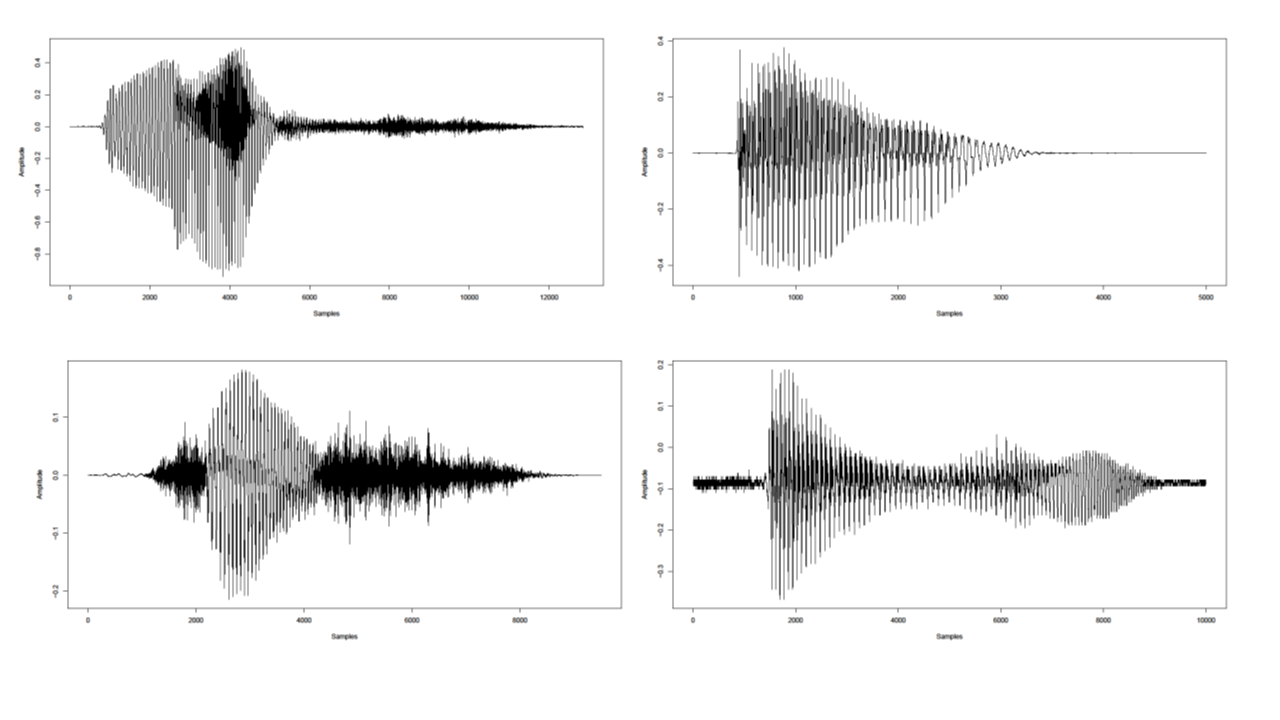
\includegraphics[width=15cm]{images/Interpolation/4 plot image.png}
    \caption{4 sample raw wave plots}
    \label{fig:4plot} 
\end{figure}

Notice the difference in length on the x-axis (the number of samples) between the four graphs. Since each of the original data has different length in time and has the same sampling rate of 1,000 Hz, the length of the data differs from one another. Thus, we have to interpolate these data prior to performing dimensional reduction.

In order to successfully implement the PCA method, we are going to apply linear interpolation on the data file. By interpolating each of the 219 acoustic signals, which were in various length, it would be compressed or lengthened to fit in the same length of 5000 data points. Each data point represents the amplitude of one millisecond of the signal, so each acoustic signals would be interpolated into a 5 second length signal with a sample rate of 1000 Hz.

The actual process of interpolation itself is simply processed by the R language built-in function \emph{approx}(), which takes in two vectors \emph{x, y}, each representing the coordinates of points to be interpolated, and an additional set of values \emph{xout}, which sets the values of points of where the interpolation would take place. The function would return two lists \emph{x, y} which represents the interpolated coordinates \cite{Approx}.

Prior to interpolation we create an empty matrix \emph{itpData} with 5,000 columns, where we would append each interpolated acoustic signals (which would be produced in vector type objects.)

For the interpolation, we create a \emph{for}() loop with variable \emph{i} going from 1 to 219, which will be representing the index for the acoustic signals of original Romance language data file. We receive each of the 219 signal data as dataframe, reconstruct it into a vector as variable \emph{y}. we also create variable \emph{x}, which is a uniformly distributed vector of length 5,000, and \emph{xoutval}, which is a uniformly distributed vector of length 5,000 from 1 to the original length of the acoustic signal. 

We then use the function \emph{approx}() with variables \emph{x, y, xoutval} and store the produced result in an object \emph{templist}. We convert the second element of obejct \emph{templist}, which is the \emph{y} component of the interpolated data, into a vector by using the built-in function \emph{unlist}(), and append it to the matrix \emph{itpData} with the built-in function \emph{rbind}().

After the \emph{for}() loop iteration we now have a matrix \emph{itpData} of 220 rows and 5000 columns (1 additional row with all 0 values, which existed as a dummy row as we initiated the matrix), where each row, except the first row, is comprised of interpolated data. We convert it into a dataframe with built-in function \emph{data.frame}() into object \emph{finalDF}, remove the first row, and finally have a dataframe \emph{finalDF} with 219 rows and 5000 columns, where each row represents the interpolated acoustic signal from the original Romance language acoustic signals.

With the 219 interpolated data we can again produce wave plots. The following figures are several examples of the wave plots.

\begin{figure}[H]
    \centering
    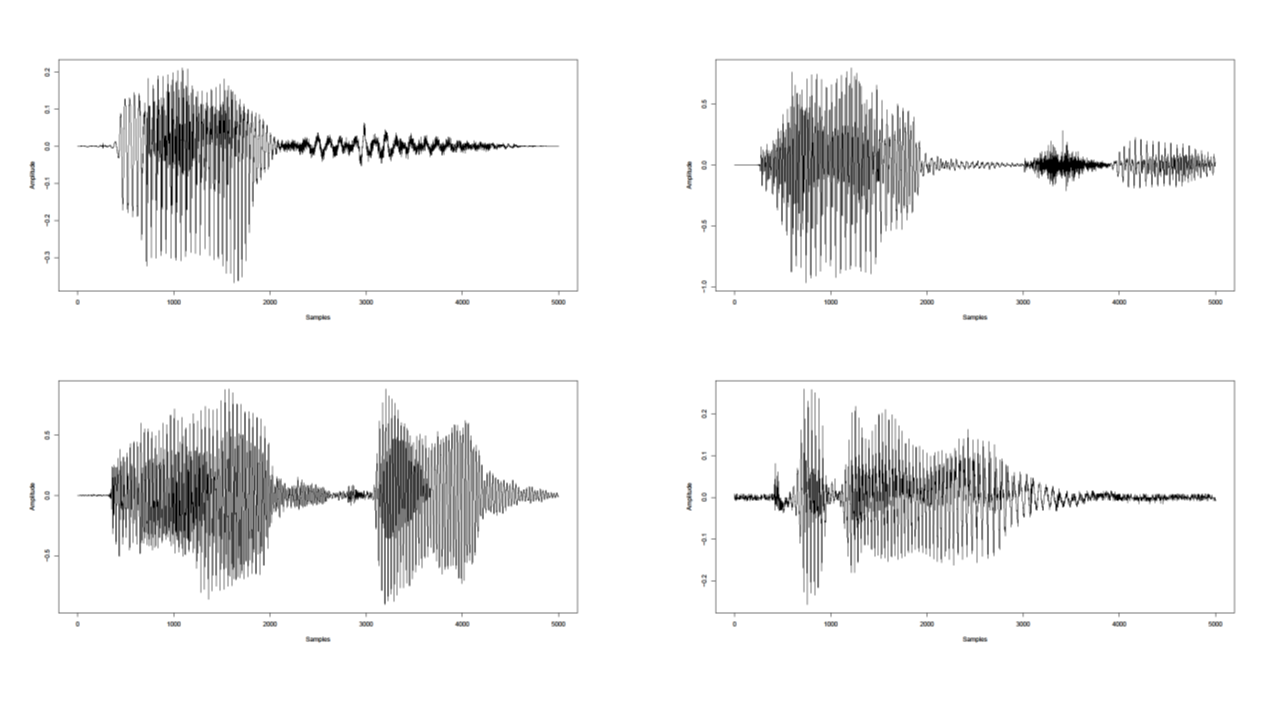
\includegraphics[width=15cm]{images/Interpolation/4 plot image (Inter).png}
    \caption{4 sample interpolated wave plots}
    \label{fig:4plotinter} 
\end{figure}

Notice that the length on the x-axis (the number of samples) of the four graphs are now fixed with 5,000 samples, as we have gone through the interpolation process. As the 219 data are aligned in same length, now the data is ready for dimensional reduction and further processing.


\newpage
\subsection{Spectrogram}


A spectrogram is a visual representation of the spectrum of frequencies of a signal as it varies over time. In other words, it shows how the energy of a signal is distributed across different frequencies at different points in time. Spectrograms are commonly used in signal processing and analysis, especially in fields like audio processing, speech recognition, and music analysis.

The basic idea behind a spectrogram is to take a signal, such as an audio recording, and divide it into short segments, typically ranging from a few milliseconds to a few seconds in length. For each segment, the spectrum of frequencies is computed using a mathematical technique called the Fourier transformation. The resulting spectrum is then displayed as a two-dimensional image, with time on the x-axis and frequency on the y-axis. The brightness or color of each pixel in the image represents the magnitude or energy of the corresponding frequency component.

By examining a spectrogram, it is possible to identify specific features of a signal that might not be apparent from the raw waveform. For example, in an audio signal, the spectrogram can reveal the presence of different harmonics and overtones, as well as variations in the amplitude and frequency content of the signal over time. Spectrograms can also be used to extract useful features for classification and recognition tasks, such as identifying different types of sounds or speech patterns.

Here is an example of a spectrogram. It is created from a sample audio file with duration of 33.5 seconds and sample rate of 8000 Hz. We read the \emph{.wav} audio file into a wave file in R with the \emph{readwave}() function in the \emph{tuneR} package. We can first plot the wave form of the file for future comparison with the spectrogram.

\begin{figure}[H]
    \centering
    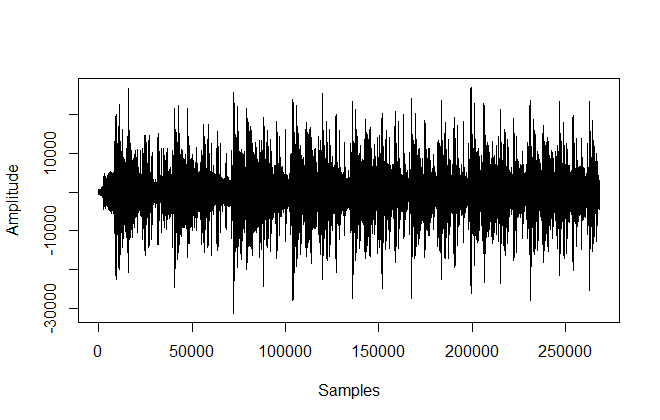
\includegraphics[width=12cm]{images/Spectrum/SampleWave.png}
    \caption{Wave form of the sample audio file}
    \label{fig:samplewave} 
\end{figure}

In order to construct a spectrogram we need to set some variable inputs. First, we shift the wave file by subtracting the mean of the signal in order to remove the DC offset. Then we set number of points to use, the window size, and the overlap. Then we can create a spectrogram with the built-in function \emph{specgram}() from the library \emph{signal}. 

The produced result \emph{spec} is a list-type data with three elements \emph{S, f, t}. Elements \emph{f} and \emph{t} are double-type objects that each represent the window size and number of points used. The element \emph{S} is a complex-type object which is the total data of the Spectrogram in a single row, having the multiplied value of \emph{f} and \emph{t} as its length.

We then go through several process on the element \emph{S} before creating a Spectrogram. We discard the phase information of \emph{S} and convert to a double-type object with function "\emph{abs}(), normalize it by dividing with the maximum amplitude \emph{max}(), and convert into dB unit by applying logarithm and multiplying by 10 unit \emph{10*log10}(). 

Now we can plot a spectrogram from the processed objects by using the built-in function \emph{imagep}() from the library \emph{oce}. We use \emph{t, f, S} as the \emph{x, y, z} component for the function \emph{imagep}() and can have the following figure as the resulting spetrogram.

\begin{figure}[H]
    \centering
    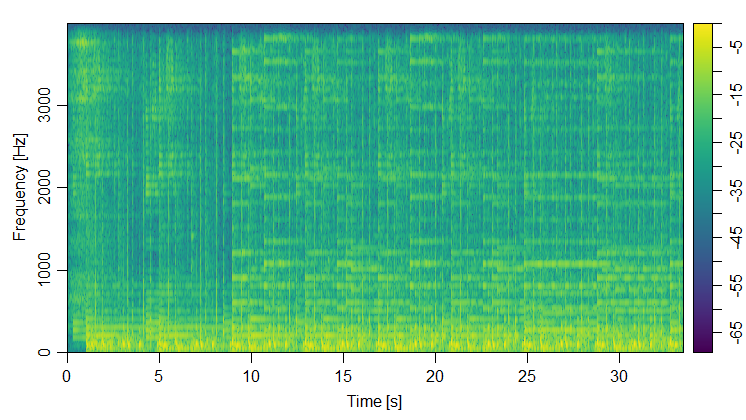
\includegraphics[width=12cm]{images/Spectrum/Spectrum (Processed).png}
    \caption{Spectrogram of the sample audio file}
    \label{fig:samplespectogram} 
\end{figure}

As we can see from the figure, Spectrograms are gnenrally a three-dimensional data set, with the third dimension displayed as colors. Time flows from left to right, which is from oldest to youngest, along the horizontal axis. The vertical axis denotes the frequency of the data, which can also be interpreted as pitch, with the lowest frequencies at the bottom and the highest frequencies at the top. The amplitude, which is also interpreted as loudness, of a particular frequency at a particular time is represented by the third dimension, color, with dark blues corresponding to low amplitudes and brighter colors up through red corresponding to progressively stronger amplitudes.

We can apply the same method of code to the interpolated dataframe of 219 acoustic signals to produce the spectrogram. We first create an empty matrix \emph{specData} with 19,456 columns (the length of the spectrogram of a single acoustic signal)  . We set the number of points to use as \emph{nfft} = 1024, widnow size as \emph{window} = 256, the overlap as \emph{overlap} = 128. Since the acoustic signals from the interpolated dataframe have 5,000 elements each, the duration and the sample rate can be set as \emph{dur} = 5 and \emph{fs} = 1,000 each.  

Now, similar to the case of interpolation, we create a \emph{for}() loop with variable \emph{i} going from 1 to 219, which will be representing the index for acoustic signals of the interpolated dataframe. We take an unlisted form of i-th row from the dataframe and store it in object \emph{snd} with the code \emph{unlist}(\emph{finalDF}[i, ]). To remove the DC offset we subtract each of 5,000 values in snd by its mean \emph{mean}(\emph{snd}). The following figure is the wave form image created from the first row of dataframe.

\begin{figure}[H]
    \centering
    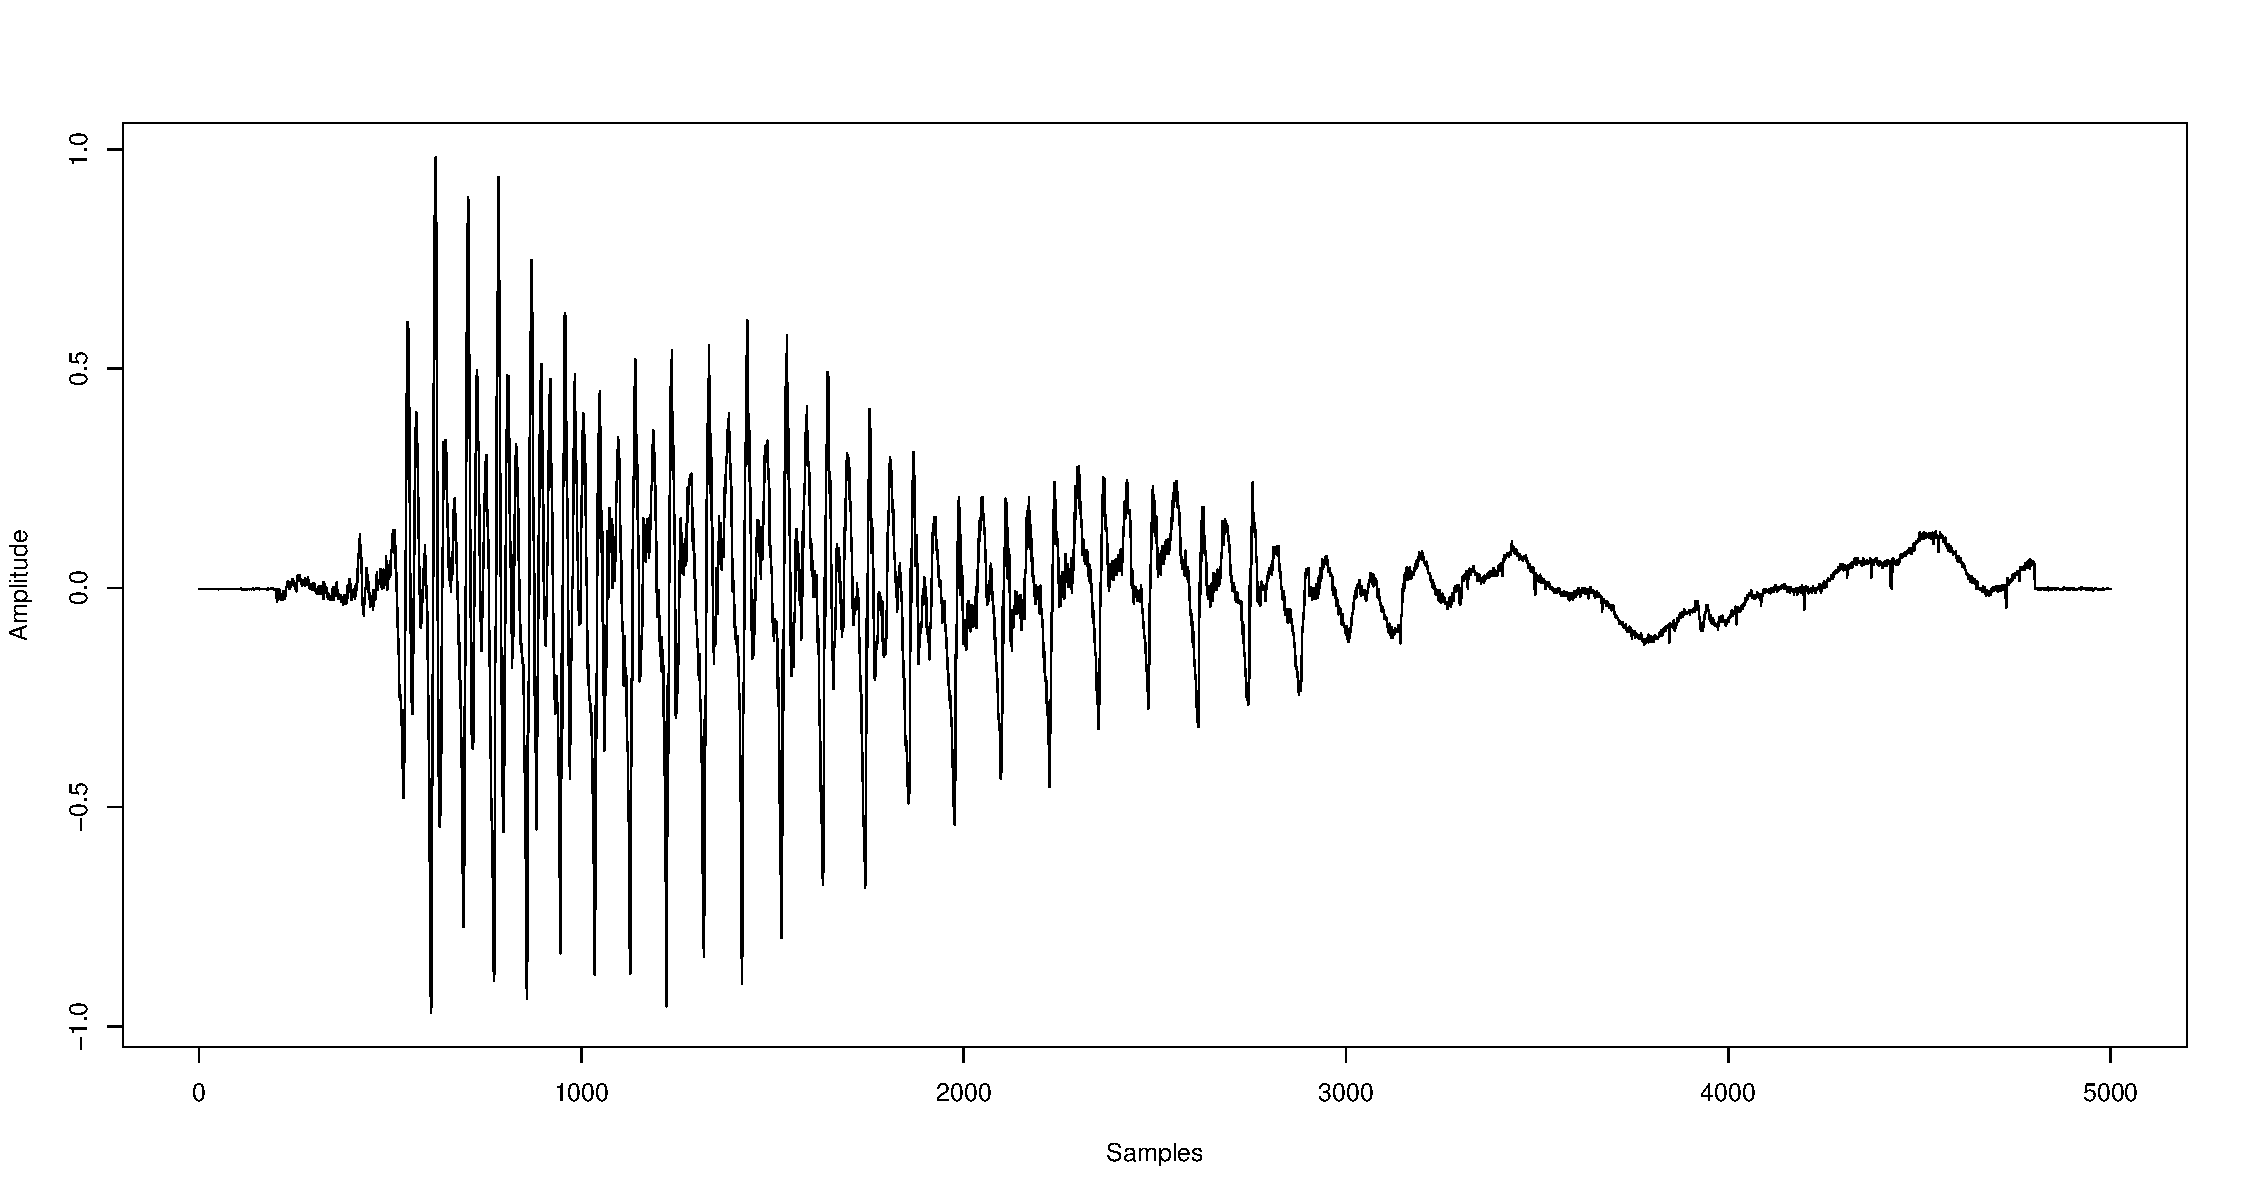
\includegraphics[width=12cm]{images/Spectrum/1RowWave.pdf}
    \caption{Wave form of the first Row of Dataframe}
    \label{fig:1RowWave} 
\end{figure}

Next, we put in the input variables \emph{snd, nfft, fs, window, overlap} into the function \emph{specgram}() and store the produced result in object \emph{spec}. We use the \emph{S} element from \emph{spec}, discard the phase information of \emph{S} with \emph{abs}(), convert to a double-type object with function "\emph{abs}(), normalize it by dividing with the maximum amplitude \emph{max}(), and convert into dB unit by applying logarithm and multiplying by 10 unit \emph{10*log10}().

Now we can plot the spectrogram by using \emph{imagep}() function and having its inputs as \emph{t, f, S} each representing the \emph{x, y, z} component. The following figure is the spectrogram image created from the first row of dataframe.

\begin{figure}[H]
    \centering
    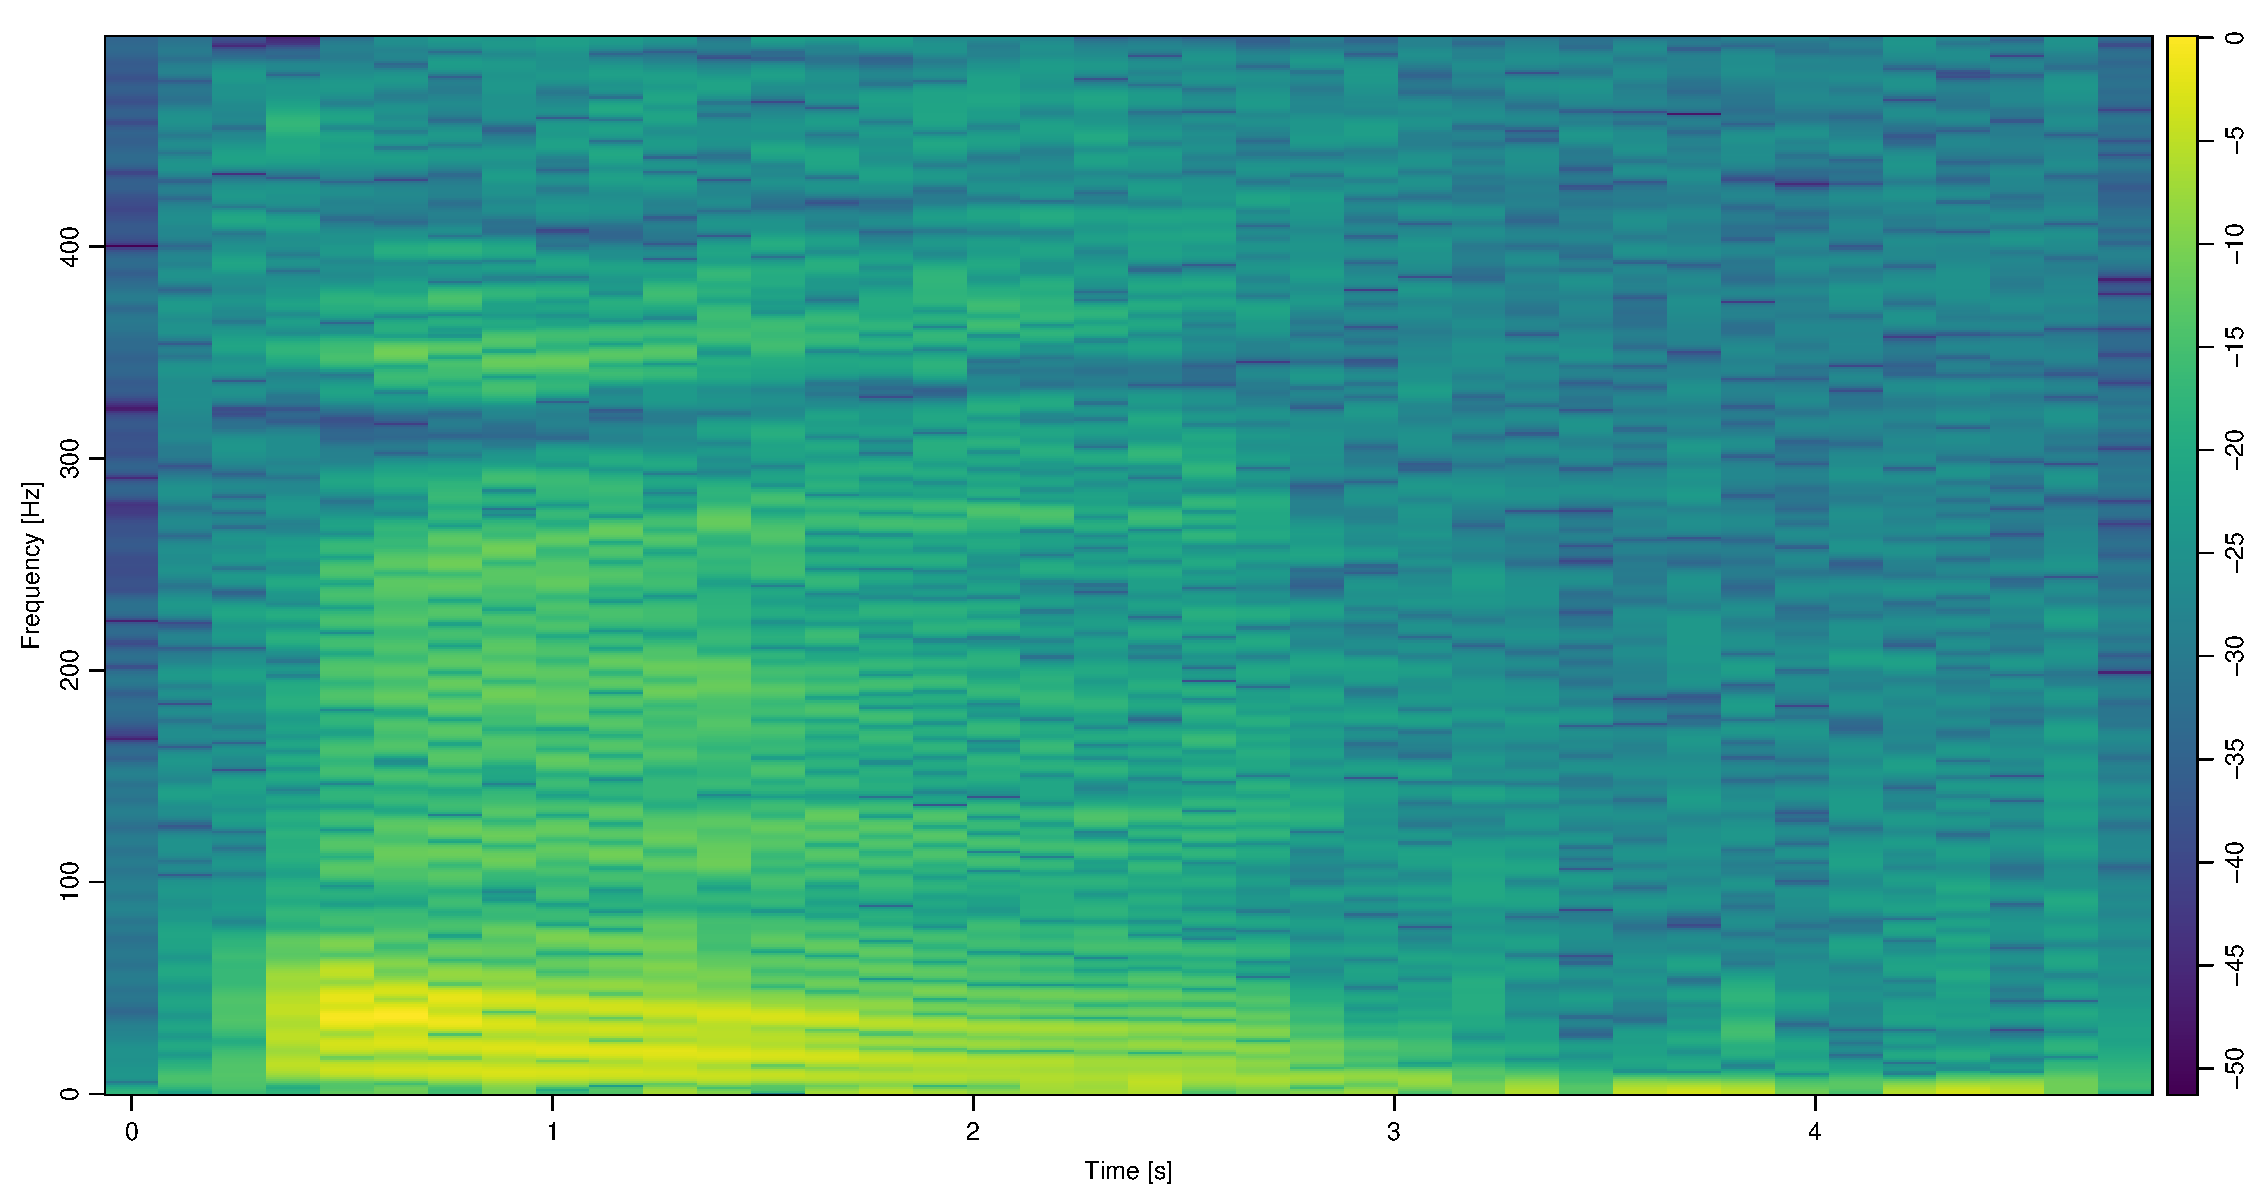
\includegraphics[width=12cm]{images/Spectrum/1Row Spec.pdf}
    \caption{Spectrogram of the first Row of Dataframe}
    \label{fig:1RowSpec} 
\end{figure}

Notice the difference in resolution compared to the example spectrogram from a sample audio file. The sample file had 33.5 seconds of duration and 8,000 Hz frequency, resulting in 33.5 * 4,000 size spectrogram (the frequency is halved as we discarded the phase information by normalizing \emph{S}), while this spectrogram has 5*500 size. The difference in the color brightness and pattern, which is the \emph{S} component from the spectrogram, shows the difference in the variance of amplitude of the two.

Finally, we can store the \emph{S} component as a row in our matrix \emph{specData} via the function \emph{rbind}().

After the \emph{for}() loop iteration we now have a matrix \emph{specData} of 220 rows and 19456 columns. We convert it into a dataframe with \emph{data.frame}() and store it into object \emph{finalSpec}, remove the first row, and finally we have a dataframe \emph{finalSpec} with 219 rows and 19456 columns, where each row correctly represents the spectrum of the original interpolated data.

